%% Results chapter
%% author Liu Peng

After designing, implementing and testing the application. We started several evaluation tests on the streaming performance. Finally we had released the application in Google Play Store in Nov 2013. So far, we have improved the application in many aspects and also brought many new features to it. During the past one year, we have accumulated many useful data and interesting results. In this chapter we will present and analyze those results.

\subsection{Performance}
In terms of streaming, our solution include two major streaming components. It would be helpful to study and compare which streaming protocol have the better performance while streaming multimedia contents. Moreover, by comparing different streaming types of media, we could investigate which protocol is best suitable for certain type of media. \\
\\Two major streaming technology we used in our solution are HTTP streaming and RTSP streaming.\\
\\
Hypertext Transfer Protocol (HTTP) refers to the protocol used to deliver web pages and images across the Internet worldwide. HTTP is an adopted, open standard and the most ubiquitous mode of delivery on-line. HTTP can be delivered by a variety of web servers, both commercial and open source.\\
\\
Real Time Streaming Protocol (RTSP) is a network control protocol used in entertainment and communications systems to control streaming media servers. RTSP is used to establish and control media sessions between two points, usually server and player client. Clients of media servers issue VCR-like commands, such as PLAY and PAUSE, to facilitate real-time control of playback of media files from the server. AirPlay uses RAOP, a RTSP-like streaming protocol, for the streaming of iTunes music. \\
\\
\textbf{Comparison of AirPlay and DLNA traffic}\\
\\
Since we have both protocols implemented in our application. We could compare the performance by streaming the same content to two receivers using different protocol, typically, DLNA music streaming uses HTTP protocol and AirPlay music streaming uses ROAP protocol. We selected a mp3 music file and try to stream it to an AirPlay Speaker and an DLNA Speaker, and we used Wireshark running on rooted Android phone to capture the packets in the network.\\
\\
After the experiment environment is set up, a series of test is conducted and the result is presented in Figure \ref{airplay_vs_dlna_traffic}.
\begin{figure}
\hfill
\subfigure[AirPlay]{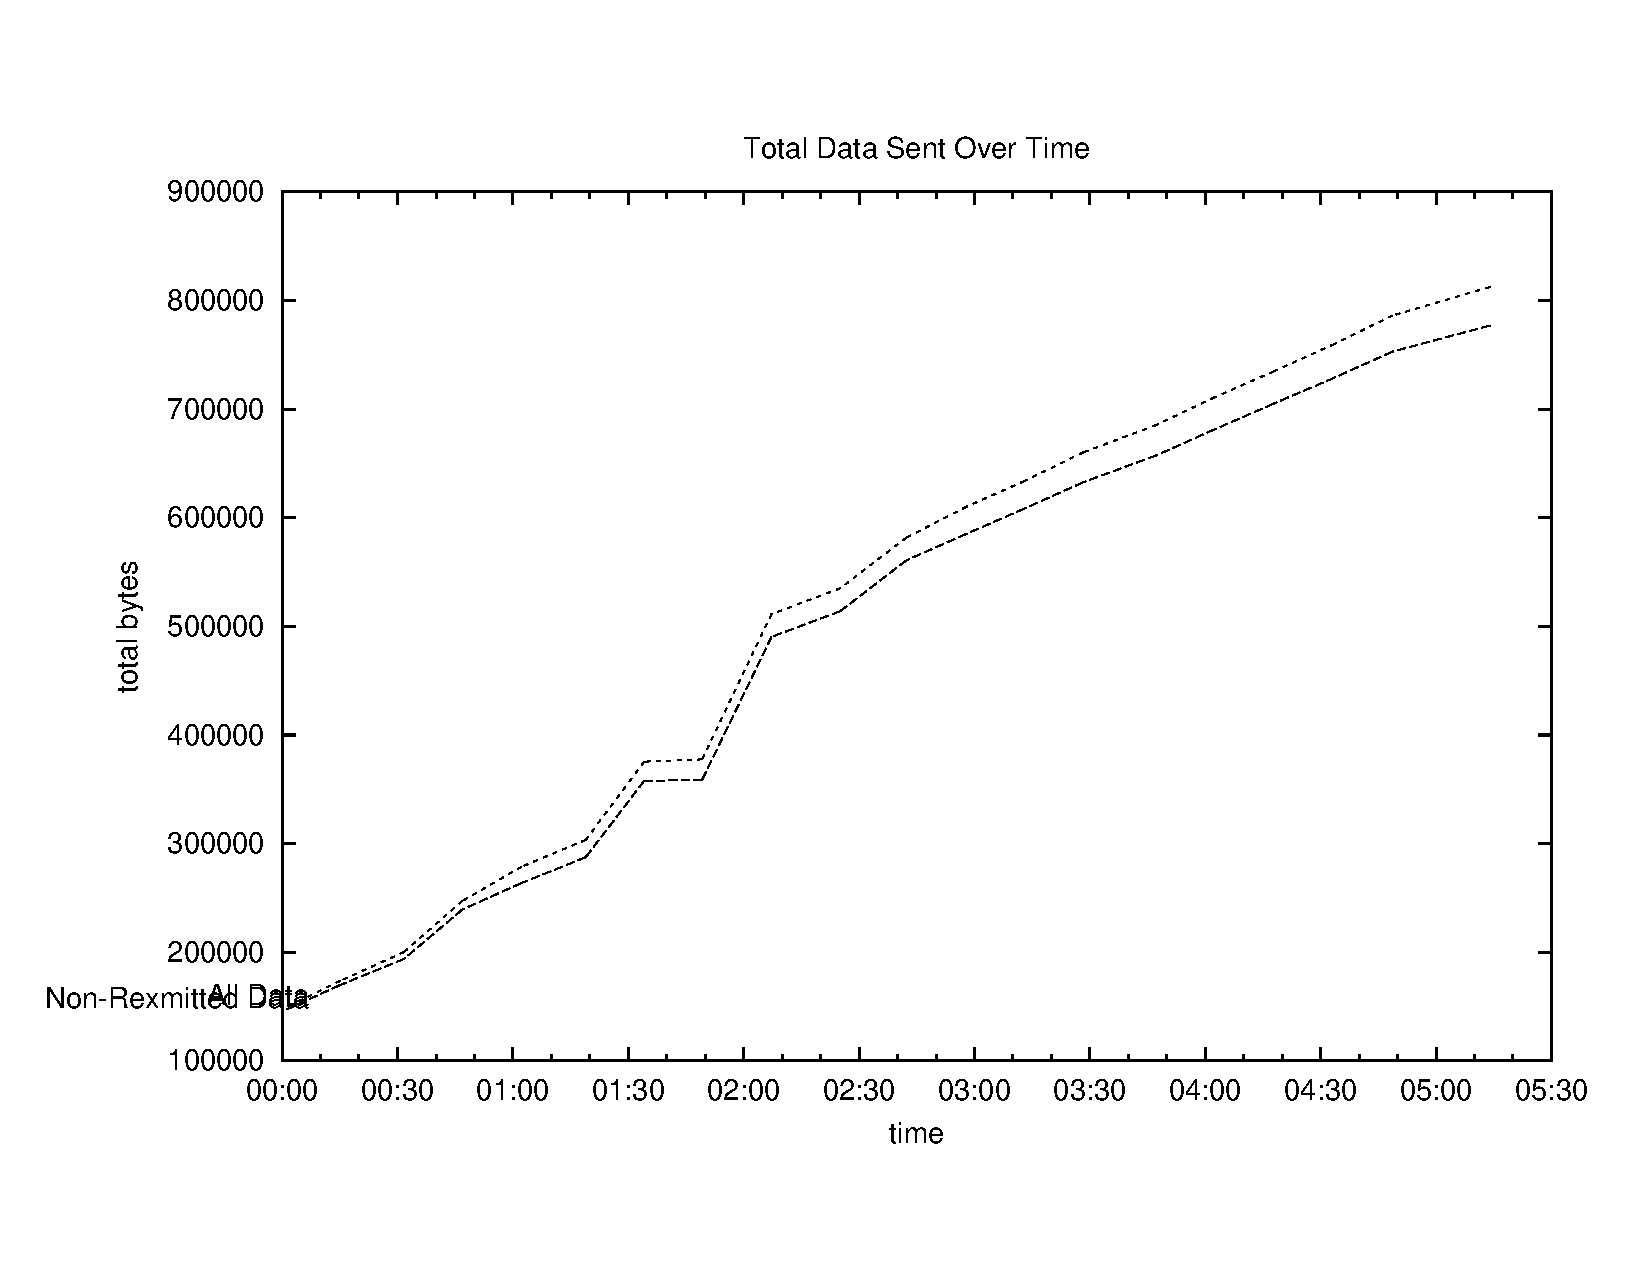
\includegraphics[width=7.2cm]{charts/oneMoreTime_airplay_android}}
\hfill
\subfigure[DLNA]{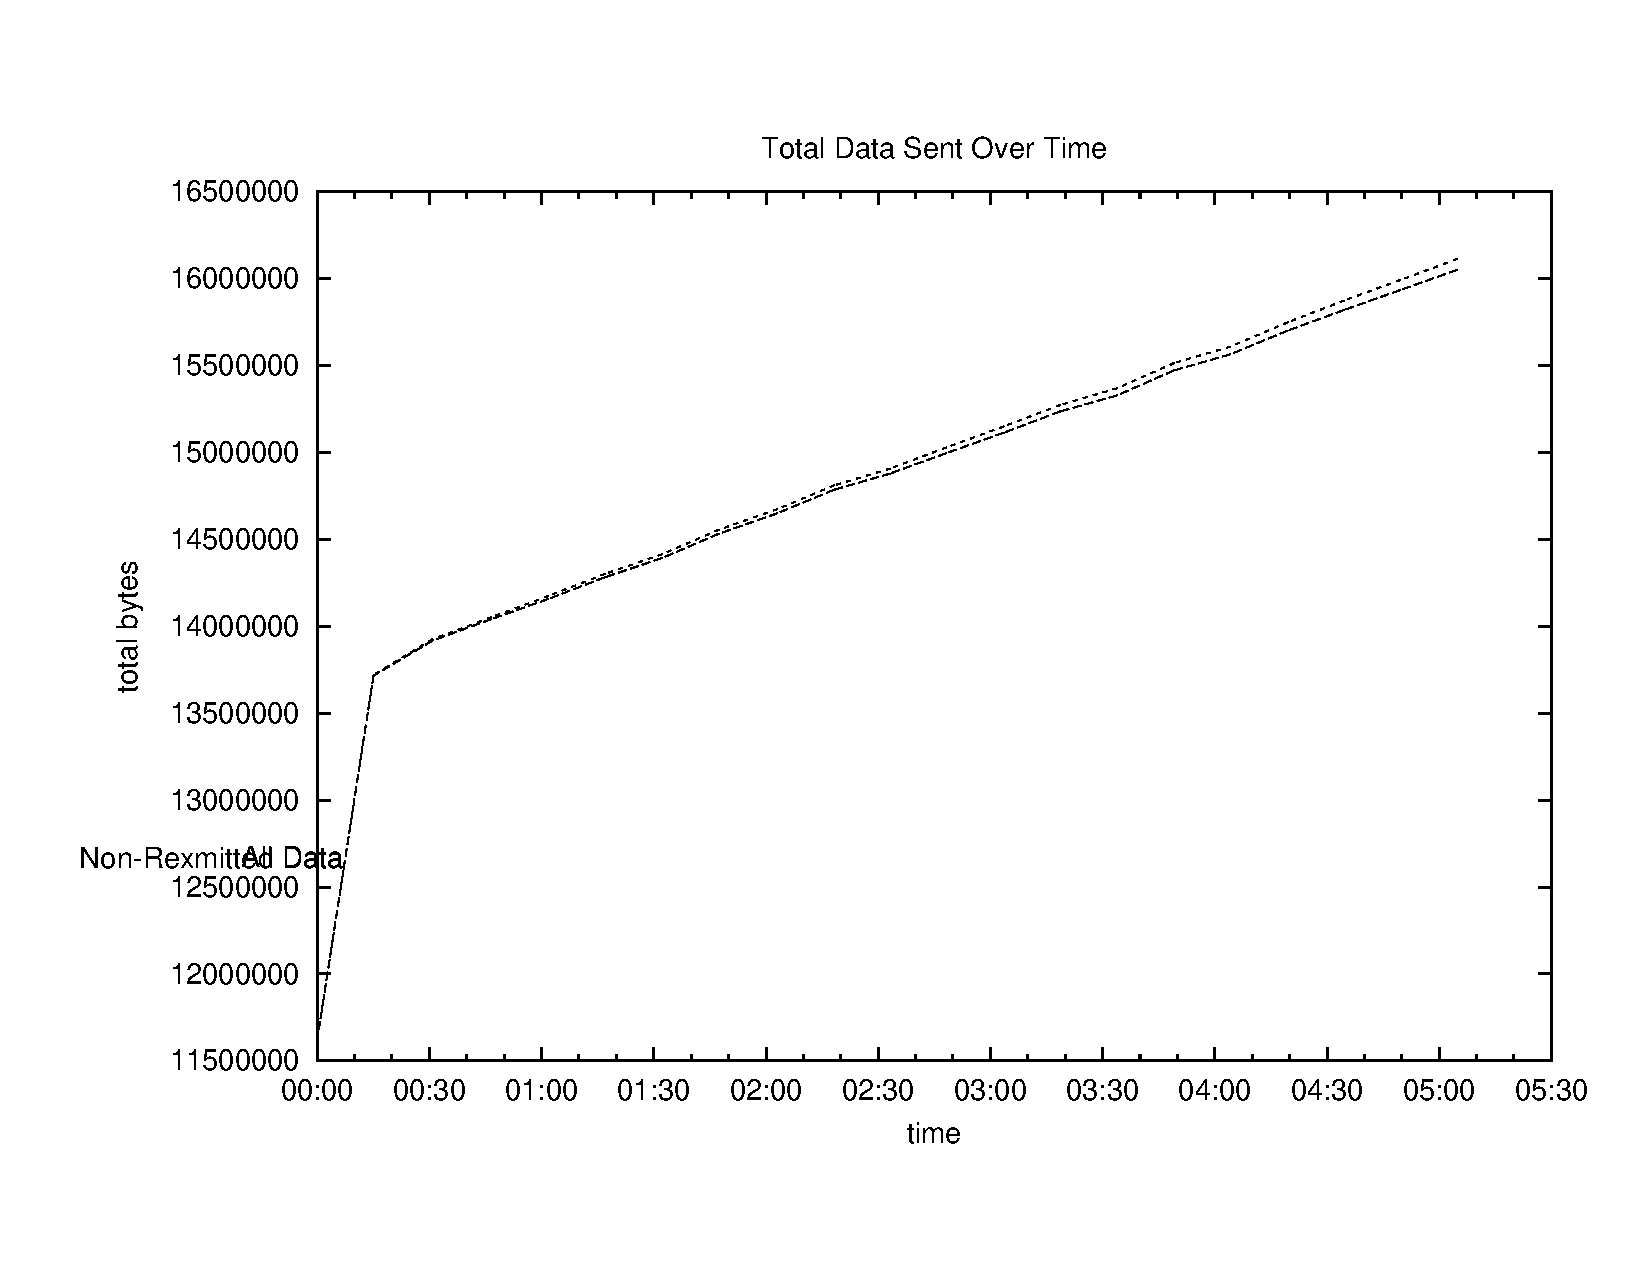
\includegraphics[width=7.2cm]{charts/oneMoreTime_dlna_android}}
\hfill
\caption{AirPlay vs DLNA streaming traffic
comparison \label{airplay_vs_dlna_traffic}}
\end{figure}
According to the figure, the stream traffic for
AirPlay and DLNA streaming is very different. For AirPlay streaming, the traffic
growth is nearly linear, because the ROAP is a push like process, content can be
streamed in real time. However, for DLNA streaming, HTTP streaming is a pull
like process, the server fetches content from media server, so the content can
be buffered at the top network speed at the beginning of the playback.
Therefore, there is a short download period at the beginning of DLNA's
graph. \\ 
\\
\textbf{Bandwidth limited situation}\\
\\
Then, we planned to limit the bandwidth and evaluate the performance change using these two solutions. We limited the bandwidth to 500 kbps, 700 kbps and 1000 kbps respectively and got Figure \ref{dlna_traffic_bw} for streaming a mp3 music to Kodi using DLNA standard.

\begin{figure}
\hfill
\subfigure[No
limit]{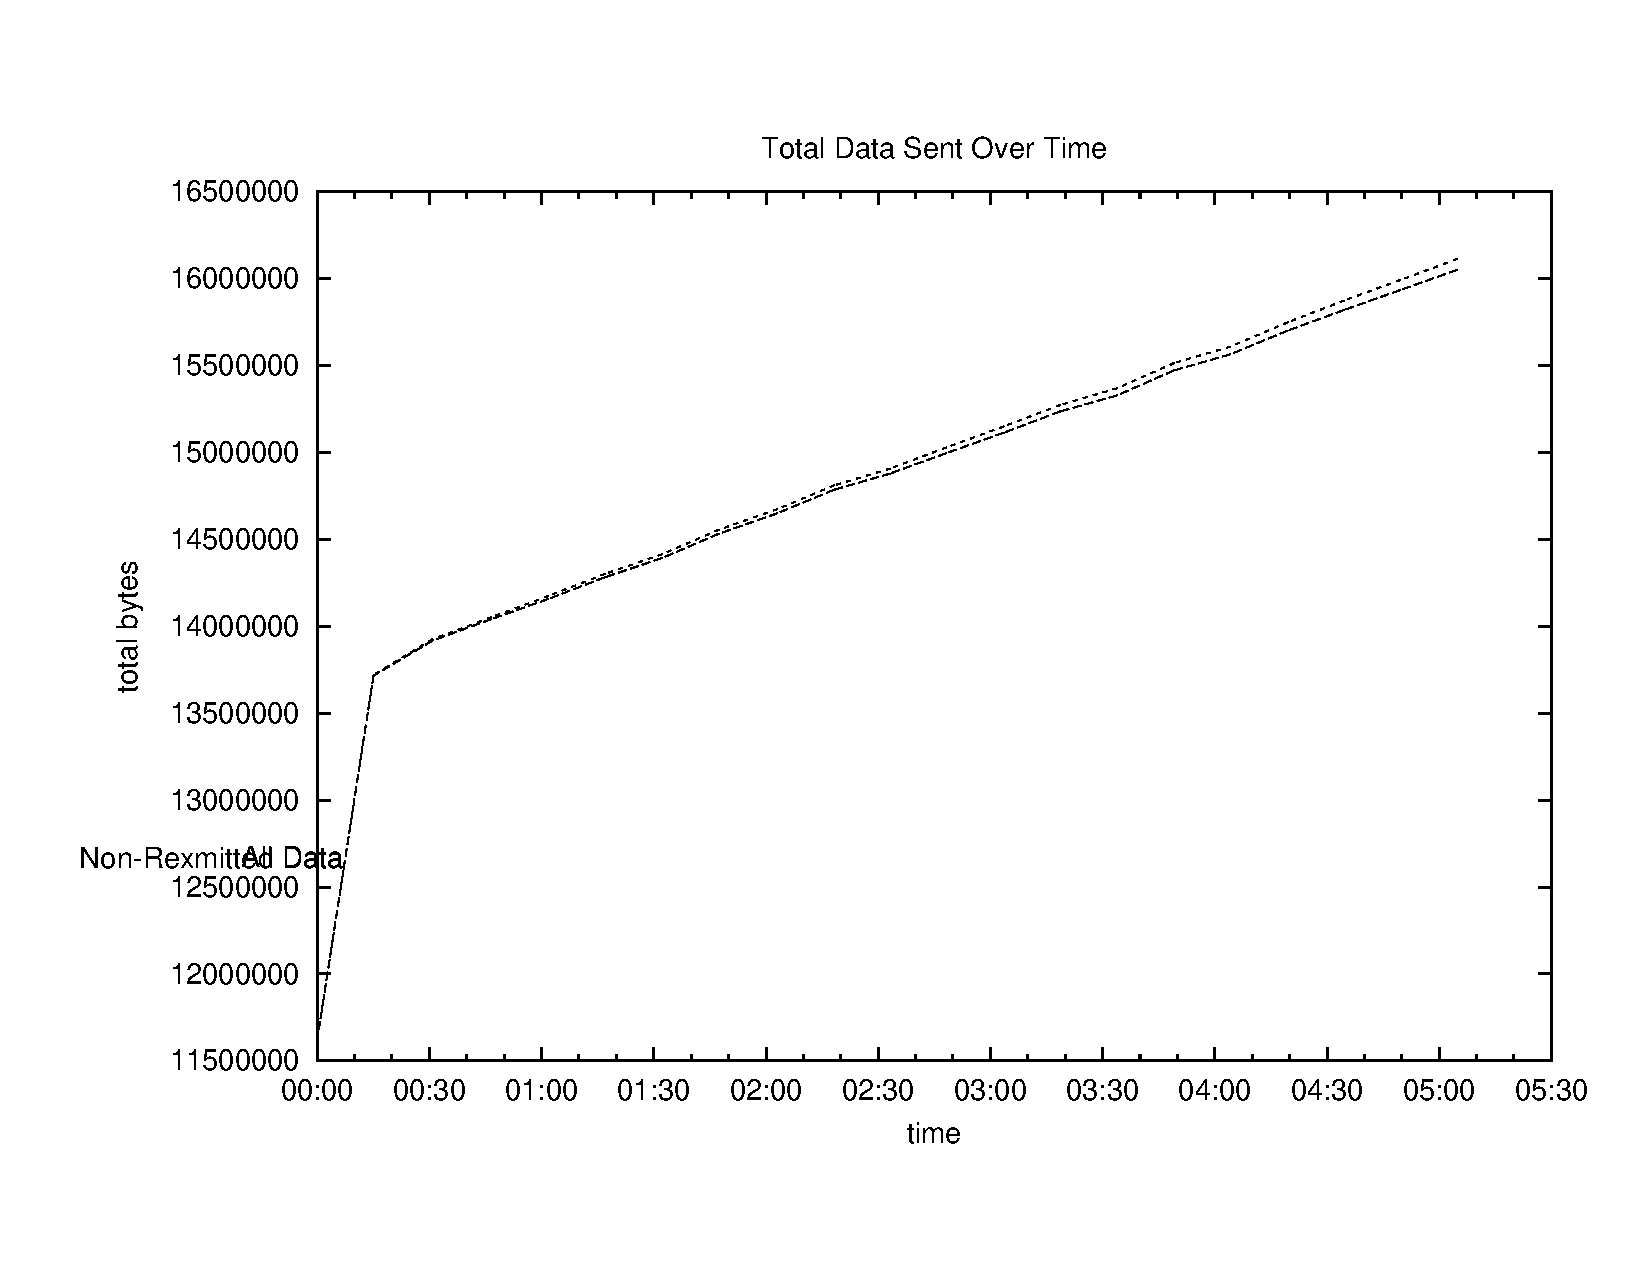
\includegraphics[width=7.2cm]{charts/oneMoreTime_dlna_android}}
\hfill
\subfigure[500kbps]{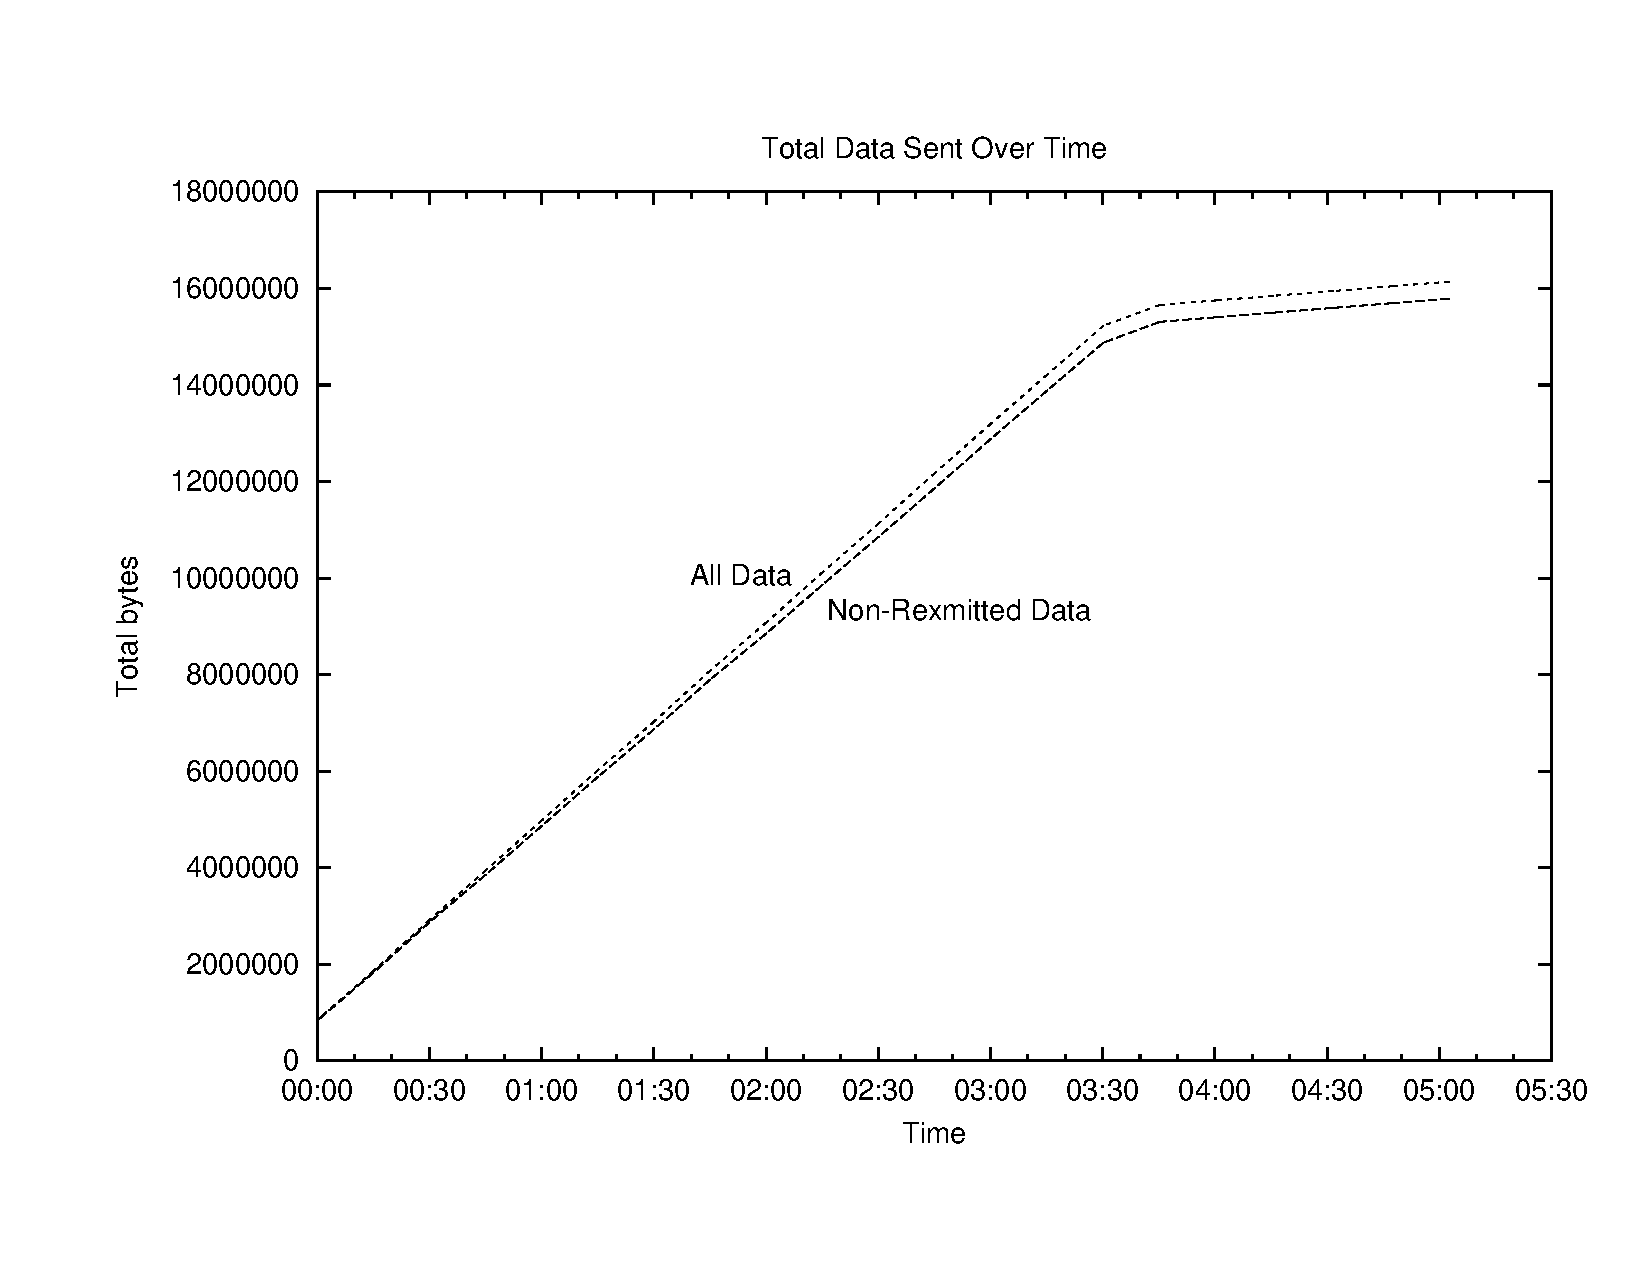
\includegraphics[width=7.2cm]{charts/oneMoreTime_dlna_android_bw_500k}}
\hfill
\subfigure[700kbps]{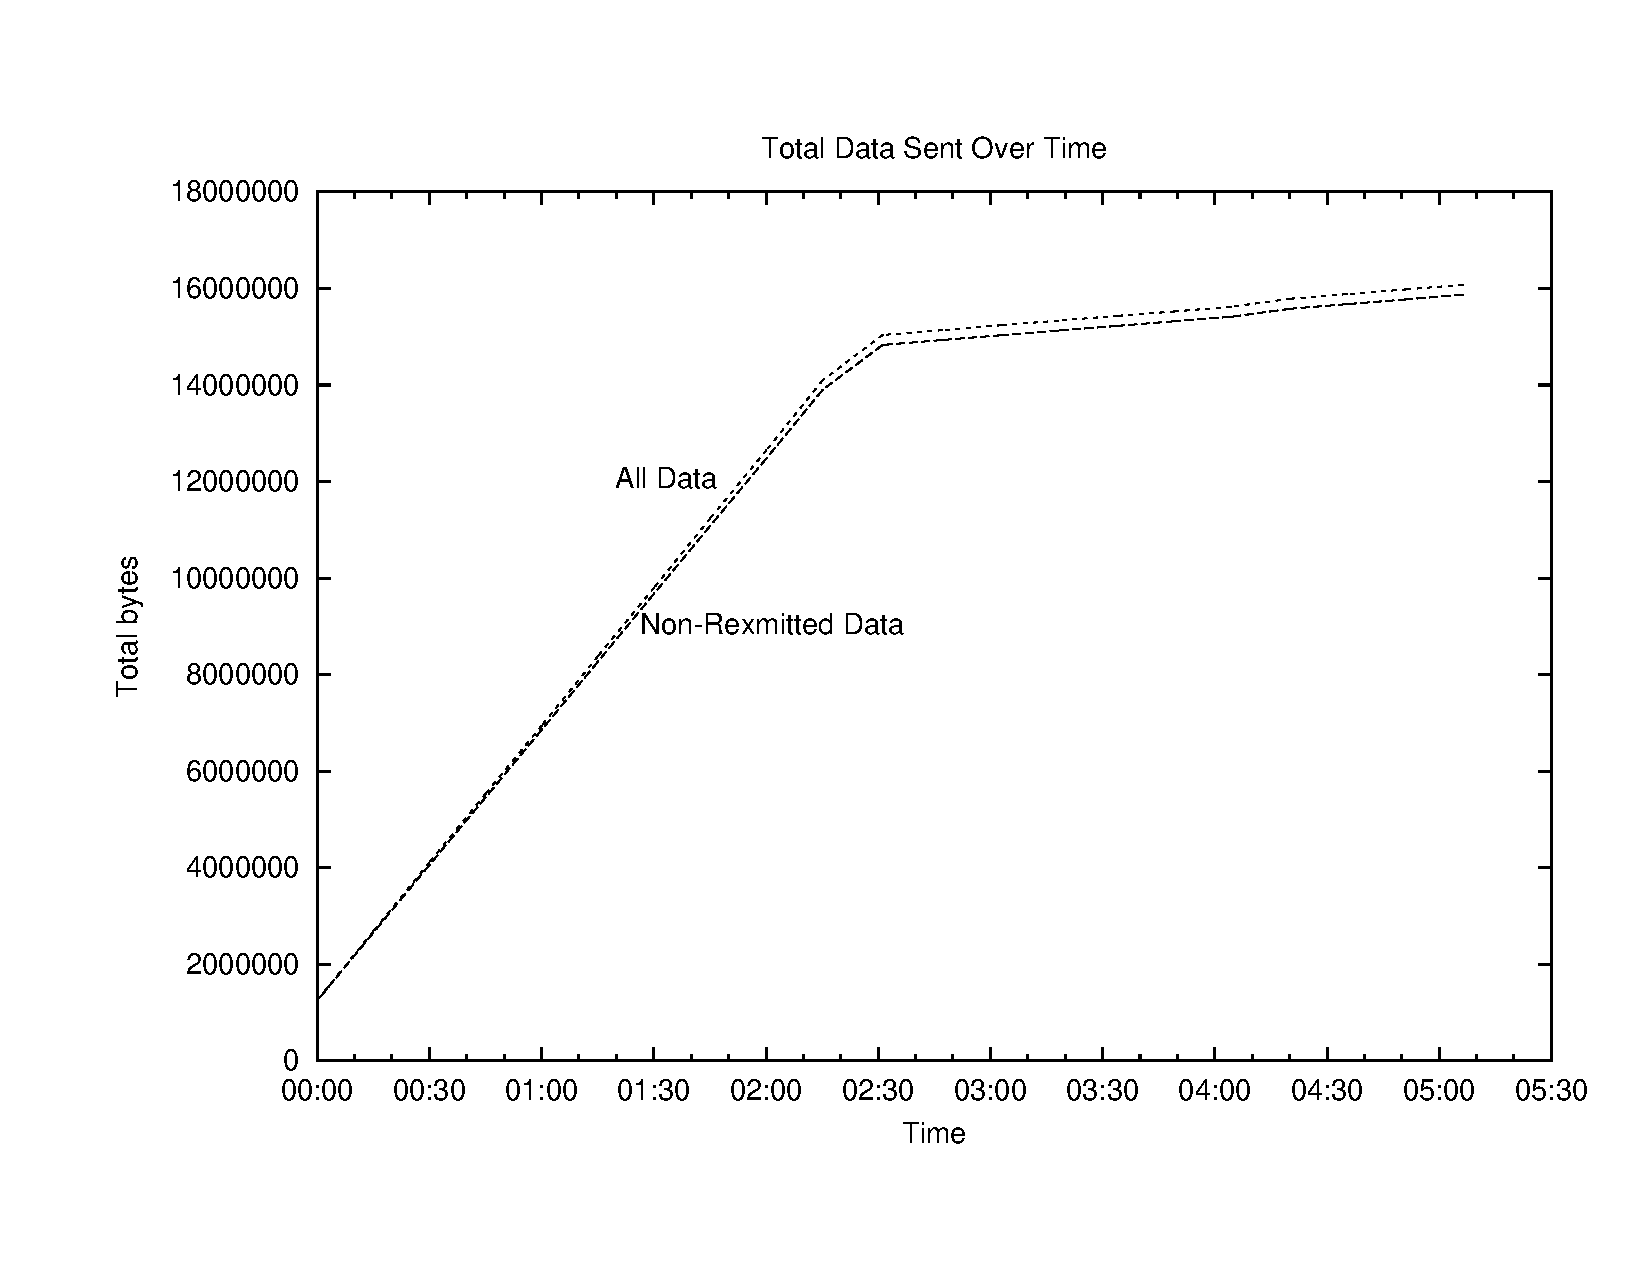
\includegraphics[width=7.2cm]{charts/oneMoreTime_dlna_android_bw_700k}}
\hfill
\subfigure[1000kbps]{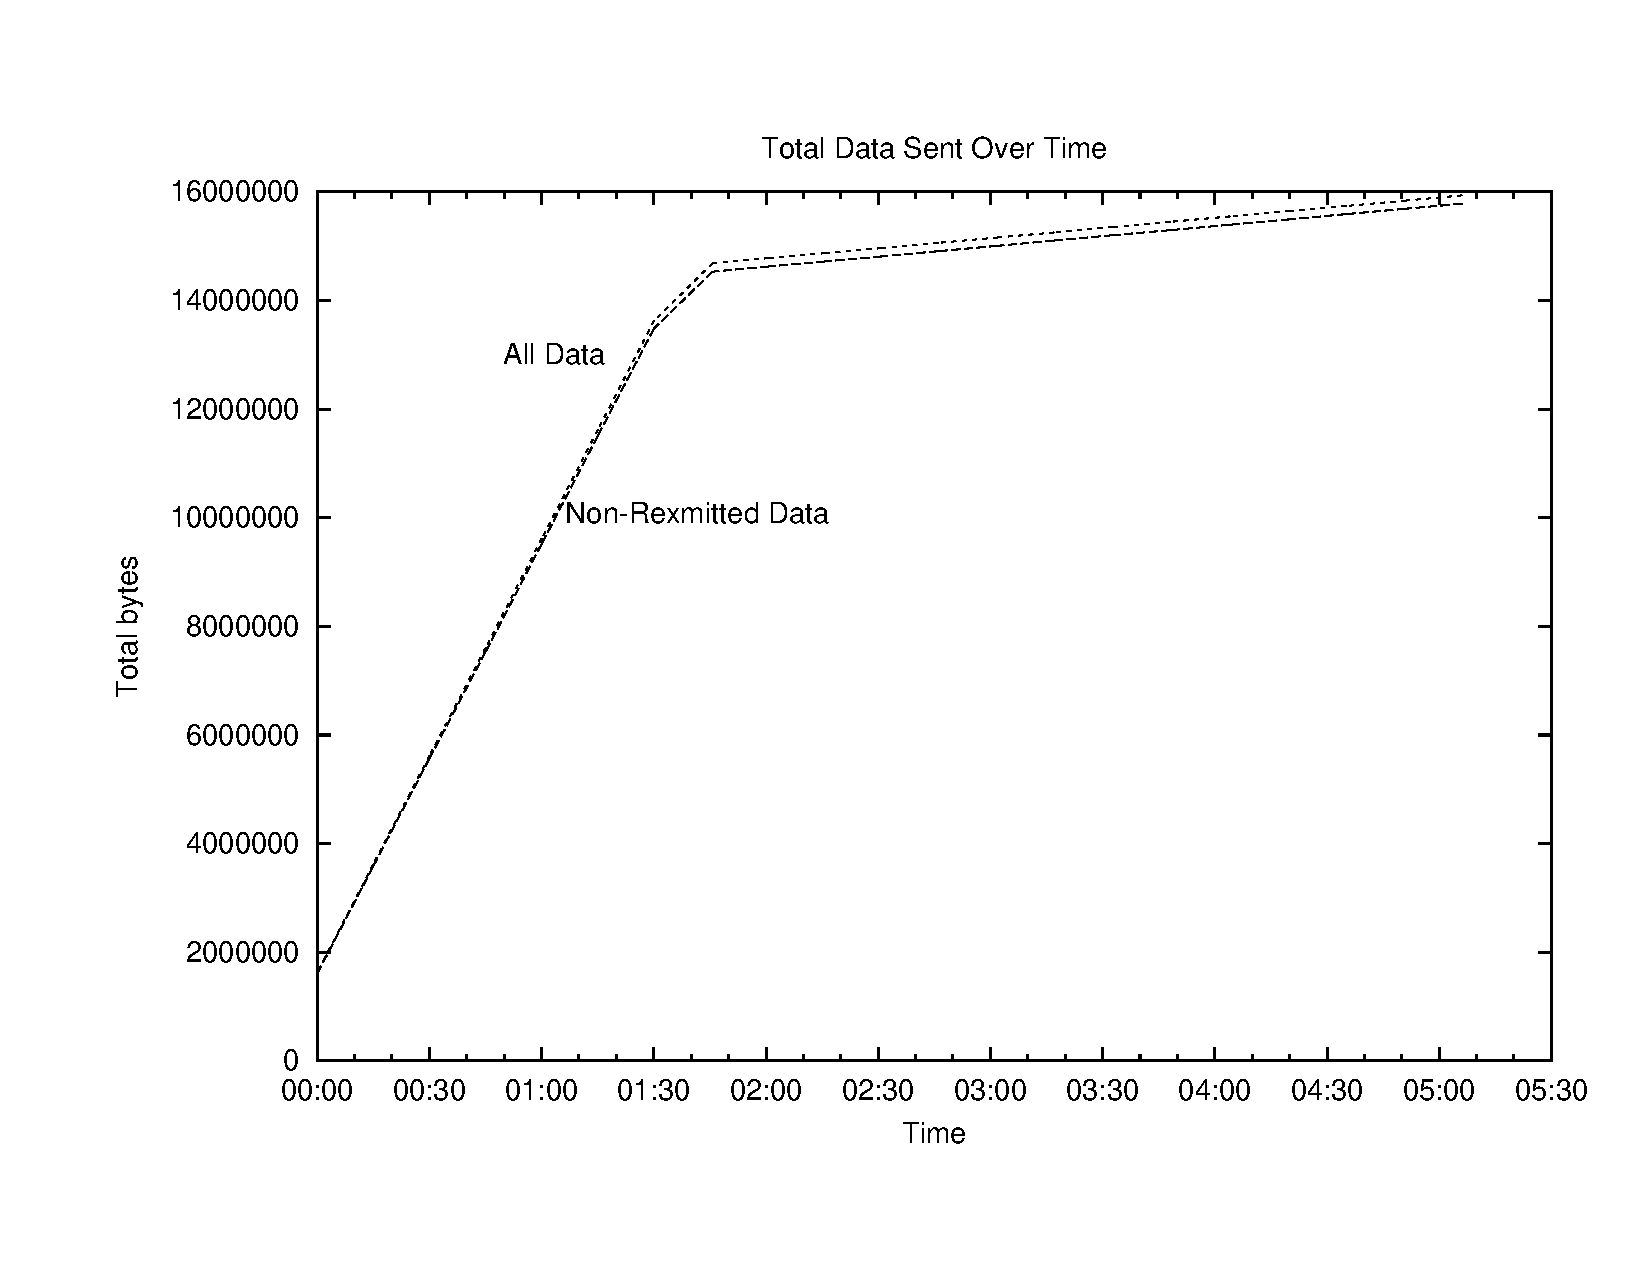
\includegraphics[width=7.2cm]{charts/oneMoreTime_dlna_android_bw_1000k}}
\hfill
\caption{DLNA streaming traffic comparison in
bandwidth constrained situation\label{dlna_traffic_bw}}
\end{figure}

According to the figure, the initial loading speed is dependent on the bandwidth of network. When there is not limit of bandwidth, the loading speed is the fastest among all the four network conditions. When the network bandwidth is limited, as the bandwidth of network increases, the initial loading speed is increasing accordingly. This proved that in DLNA streaming, since HTTP streaming is used, most of the content is fully downloaded in the initial phase of streaming. The quality of steaming can be guaranteed when the initial buffer is finished. The receiver will take the buffered content and play locally.\\
\\
On the other hand, AirPlay music streaming is based on ROAP, which is a RTP-like protocol. The transport layer protocol used is UDP, thus not all packets can be delivered to the receiver, it is a best-effort transmission. The sound quality can not be guaranteed because there is no buffer or retransmission mechanism on the receiver side, the transmission is almost real-time. Given this reason, when the bandwidth is limited to 500 kbps, the AirPlay playback is heavily interrupted, all music information is lost since the too many packets are lost during the transmission. When the bandwidth is increased to 700 kbps, the AirPlay playback still can not work properly, the playback is cut and choppy. After the bandwidth is increased to 1000 kbps, the music can work properly and basically no noise can be heard.\\
\\
Another thing worth mentioning is that in the experiment, same mp3 music is used in both tests. But obviously the playback quality of DLNA is better than the playback using AirPlay. For instance, when the bandwidth is limited to 500 kbps, AirPlay streaming is basically not useable any more, while DLNA streaming is still working properly. The reason behind this is that in the case of DLNA streaming, the original mp3 music is directly streamed to receiver, while in the case of AirPlay music streaming, the same mp3 music is firstly decoded to PCM format and then encoded to Apple Lossless format. Since mp3 is a compressed media format while Apple lossless format is an uncompressed media format, the bandwidth required for DLNA streaming is considerably smaller than AirPlay streaming.\\
\\
Generally speaking, DLNA is more tolerant than AirPlay streaming in case of limited bandwidth.\\
\\
\textbf{Influence of packet loss}\\
\\
Next step, we simulated packet loss on the receiver side and conduct the same test for DLNA and AirPlay streaming. 5\%, 10\% and 15\% packet loss are adopted separately for DLNA and AirPlay streaming. The result of DLNA streaming is shown in Figure \ref{dlna_pl}. \\
\begin{figure}
\hfill
\subfigure[No
limit]{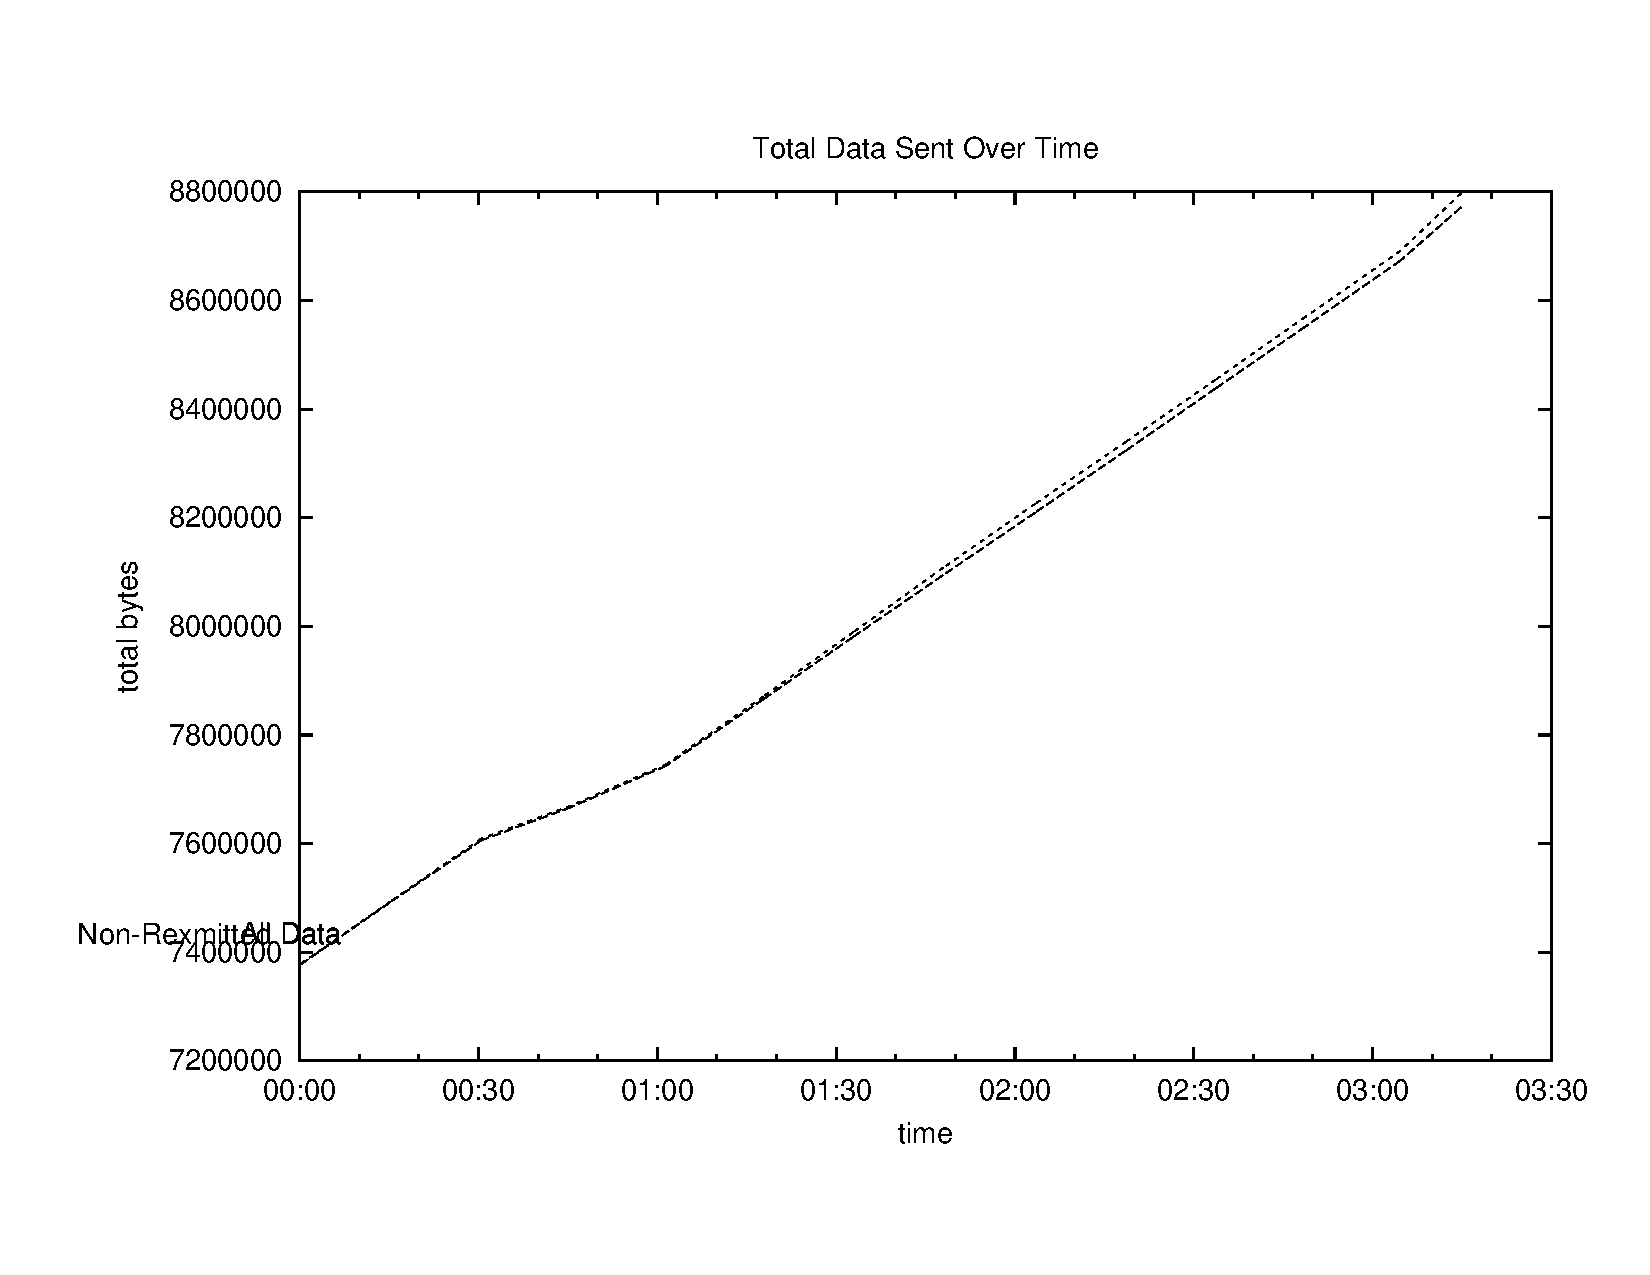
\includegraphics[width=7.2cm]{charts/dlna_traffic_data}}
\hfill
\subfigure[5
percent loss]{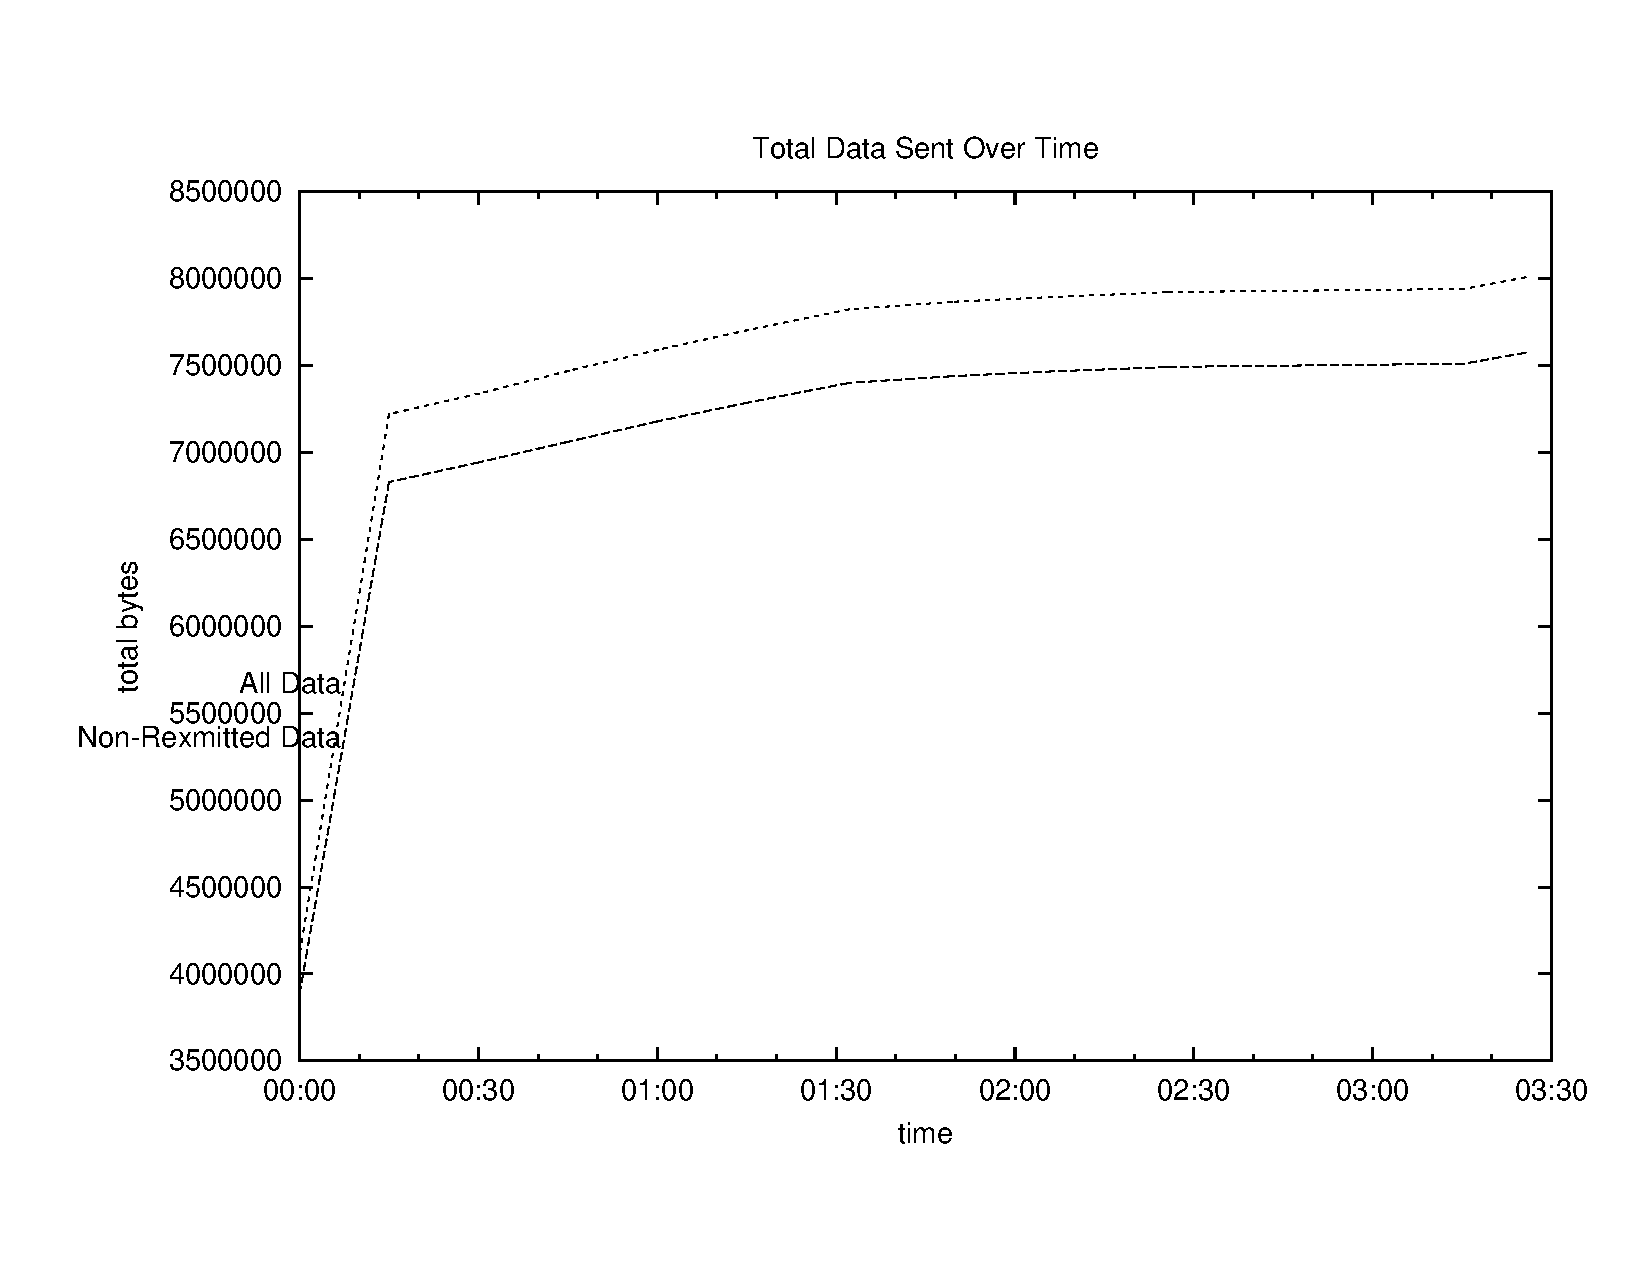
\includegraphics[width=7.2cm]{charts/dlna_traffic_5loss_data}}
\hfill
\subfigure[10
percent loss]{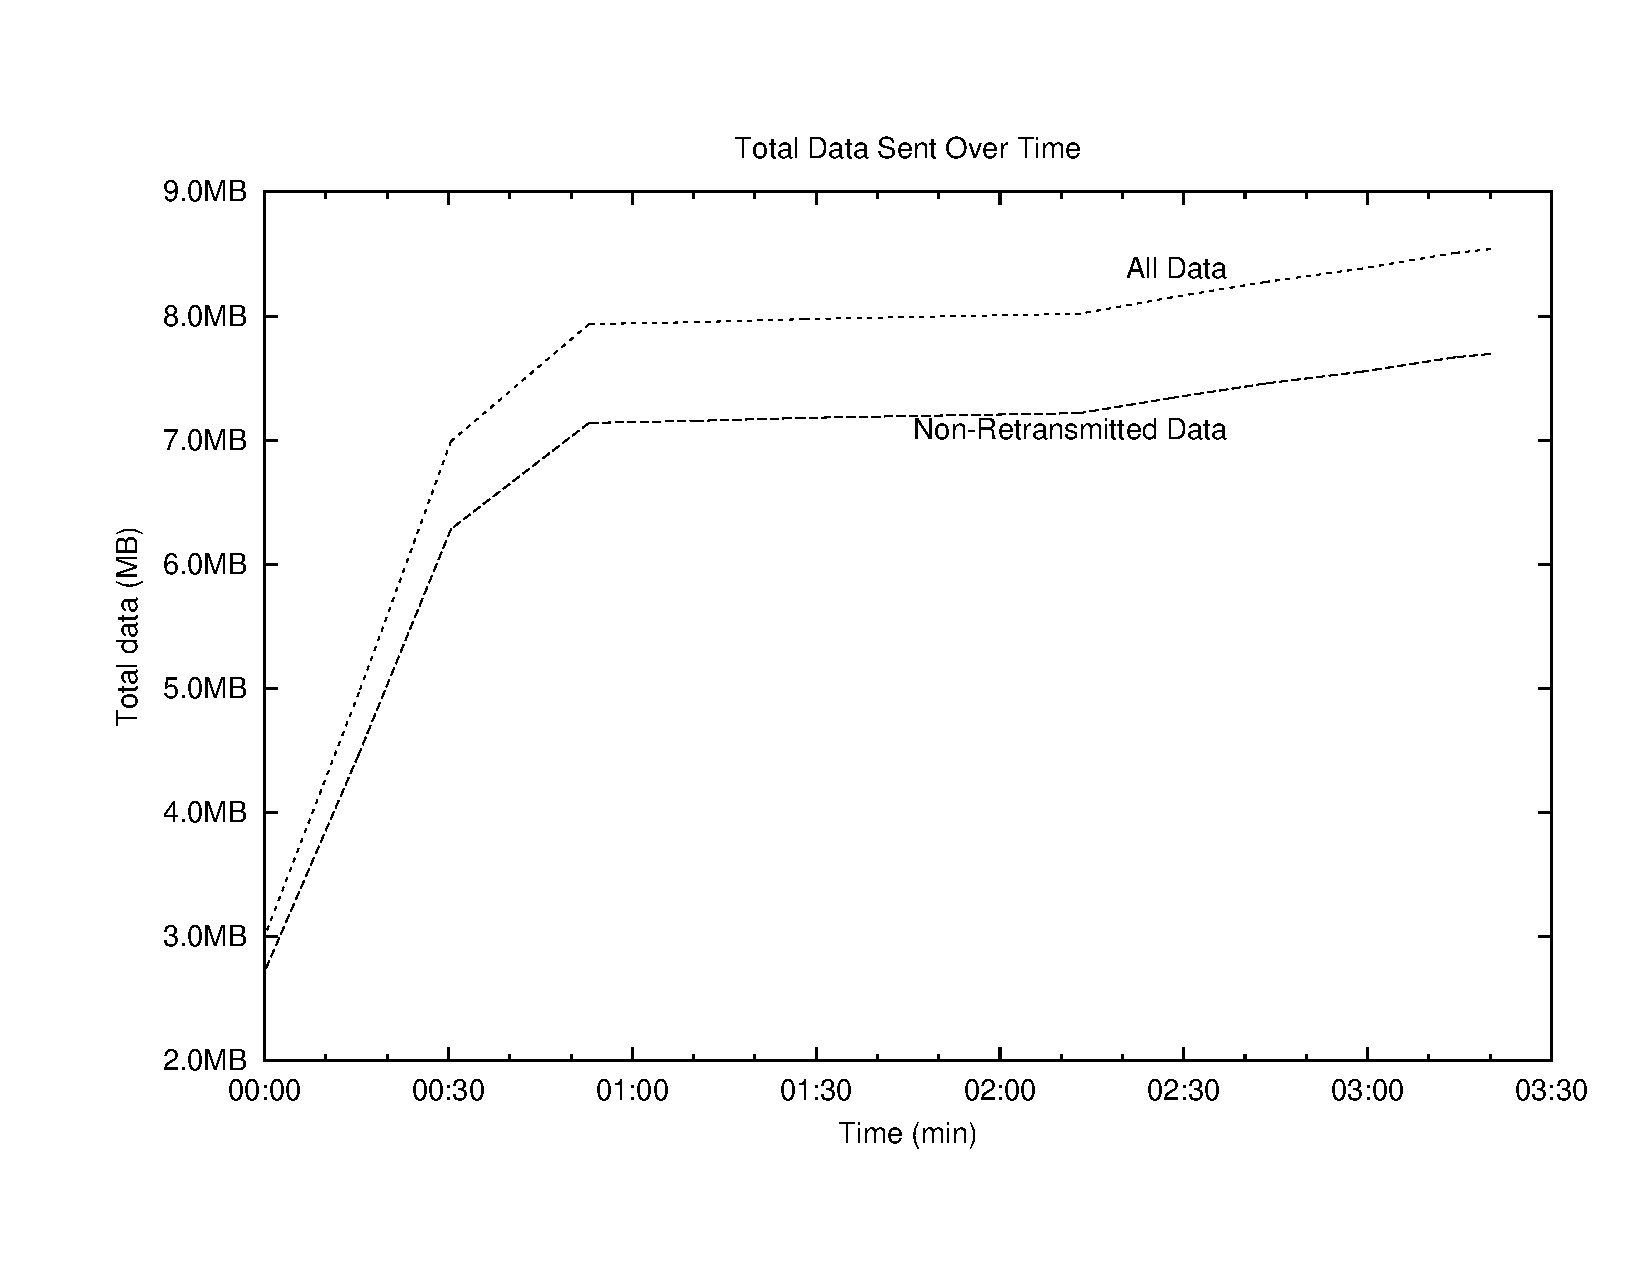
\includegraphics[width=7.2cm]{charts/dlna_traffic_10loss_data}}
\hfill
\subfigure[15
percent loss]{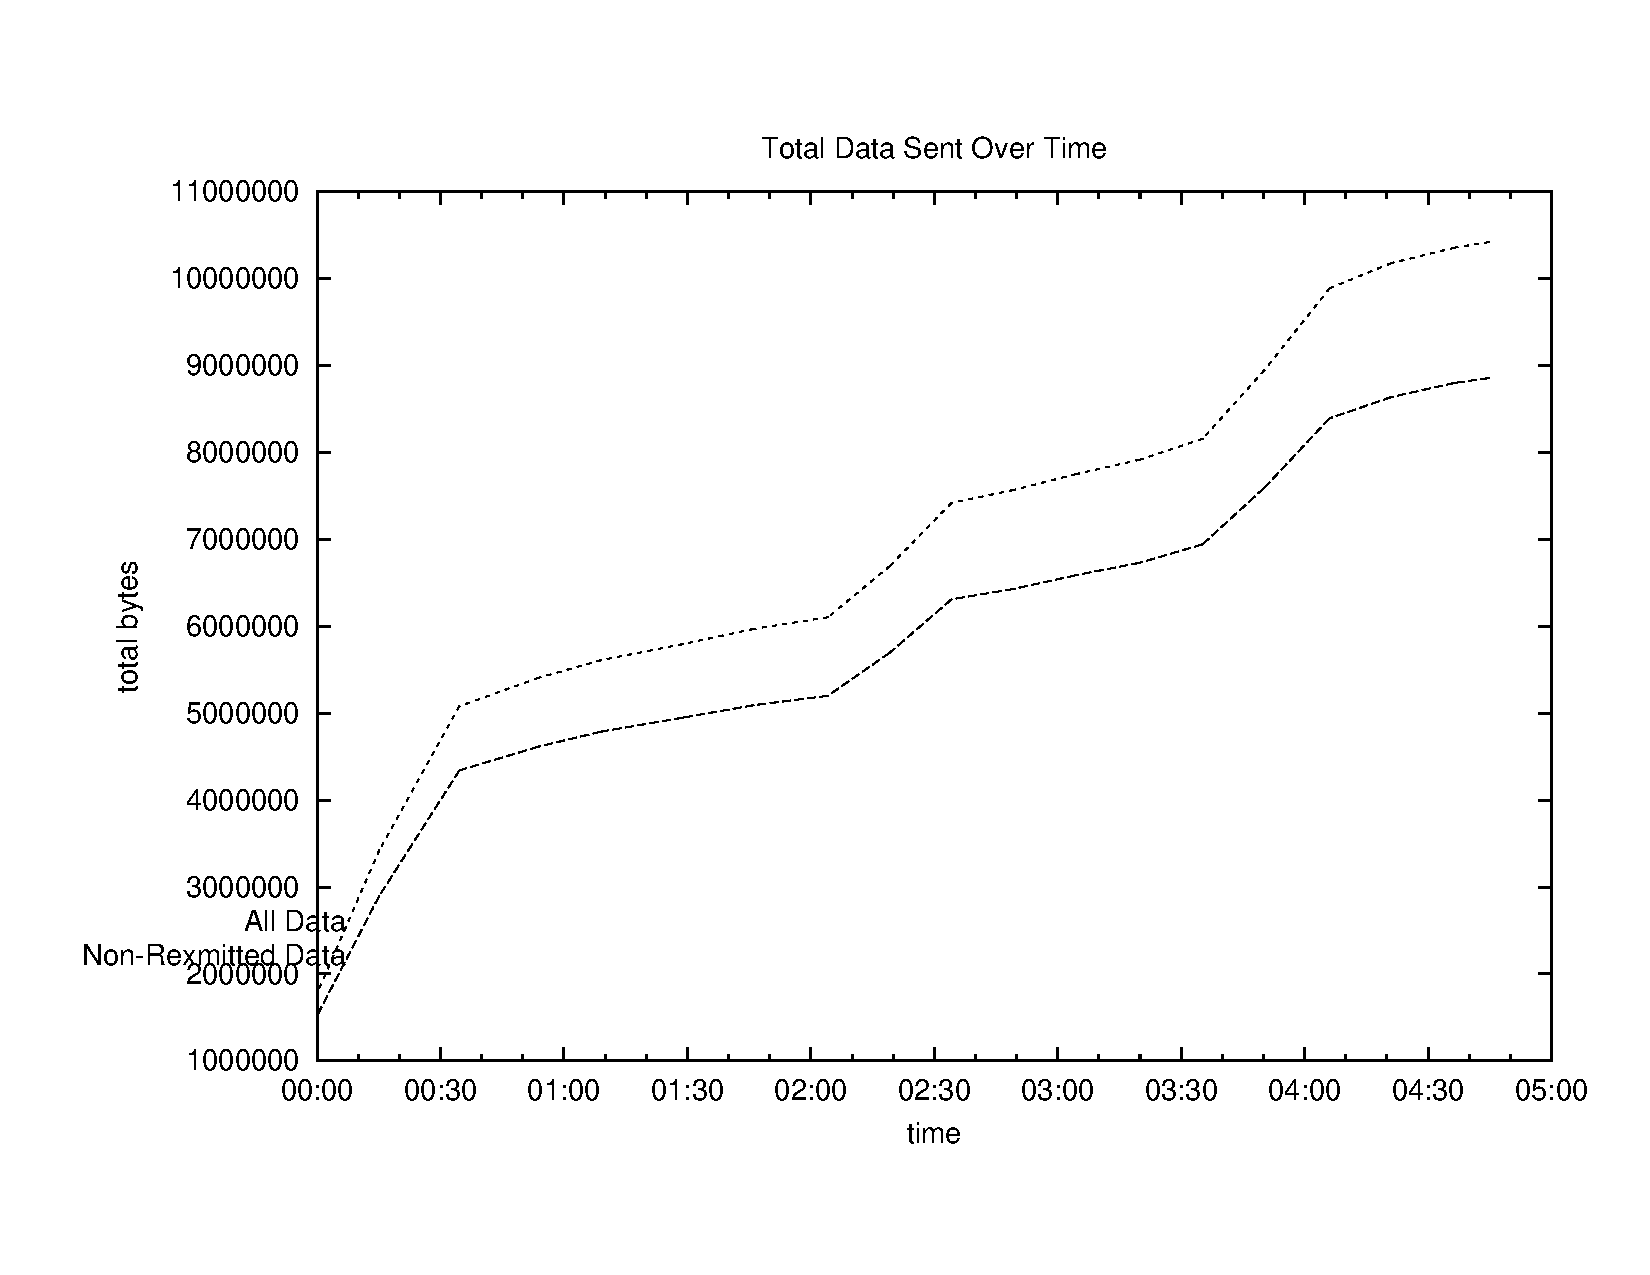
\includegraphics[width=7.2cm]{charts/dlna_traffic_15loss_data}}
\hfill
\caption{DLNA streaming performance in terms of packet loss \label{dlna_pl}}
\end{figure}
\\
According to the figure, when there is not packet loss, very little retransmission data is seen in the graph. When the packet loss ratio is increased from 5\% to 10\%, the portion of retransmitted data is getting larger and larger, however, there is no noticeable loss of sound quality. But when the packet loss ratio is increased to 15\%, significant amount of retransmission can be found in the graph, and the streaming is cut and wait for buffering three times during one song's playback. In the case of DLNA streaming, packet loss is a key impediment for streaming, when packet loss get worse enough, for instance, in our experiment, 15\% packet loss will make the streaming unusable.\\
\\
On the other hand, same experiment with AirPlay streaming was conducted, and the results which is shown in Figure \ref{airplay_pl}. According to the figure, in the case of AirPlay streaming, since UDP is used for music streaming, the ROAP server embedded in Streambels keeps sending data to receiver using UDP regardless of packet loss. On the receiver side, the player tries its best to decode the broken data. There is no mechanism for acknowledgement or retransmission. Surprisingly, the sound quality is much better compared with DLNA streaming. The reason behind is that retransmission of TCP mechanism consumes more and more bandwidth in the case of DLNA streaming, in the same situation, AirPlay streaming tries to deliver all contents in its best effort.\\
\\
Totally speaking, in the case of packet loss, AirPlay is more tolerant than DLNA standard.
\begin{figure}
\hfill
\subfigure[No
limit]{\includegraphics[width=7.2cm]{charts/AirPlay_traffic_data}}
\hfill
\subfigure[5
percent loss]{\includegraphics[width=7.2cm]{charts/AirPlay_traffic_5loss_data}}
\hfill
\subfigure[10
percent loss]{\includegraphics[width=7.2cm]{charts/AirPlay_traffic_10loss_data}}
\hfill
\subfigure[15
percent loss]{\includegraphics[width=7.2cm]{charts/AirPlay_traffic_15loss_data}}
\hfill
\caption{AirPlay streaming performance in terms of packet loss \label{airplay_pl}}
\end{figure}


\subsection{Statistics}
Through 16 months' releasing, our application have achieved 924000 downloads from 223 countries all around the world, with around 10000 daily active users. This means our users almost cover 99\% of the earth, a world map of our users is shown in Figure \ref{user_map}. \\
\\
\begin{figure}[htb]
\centering 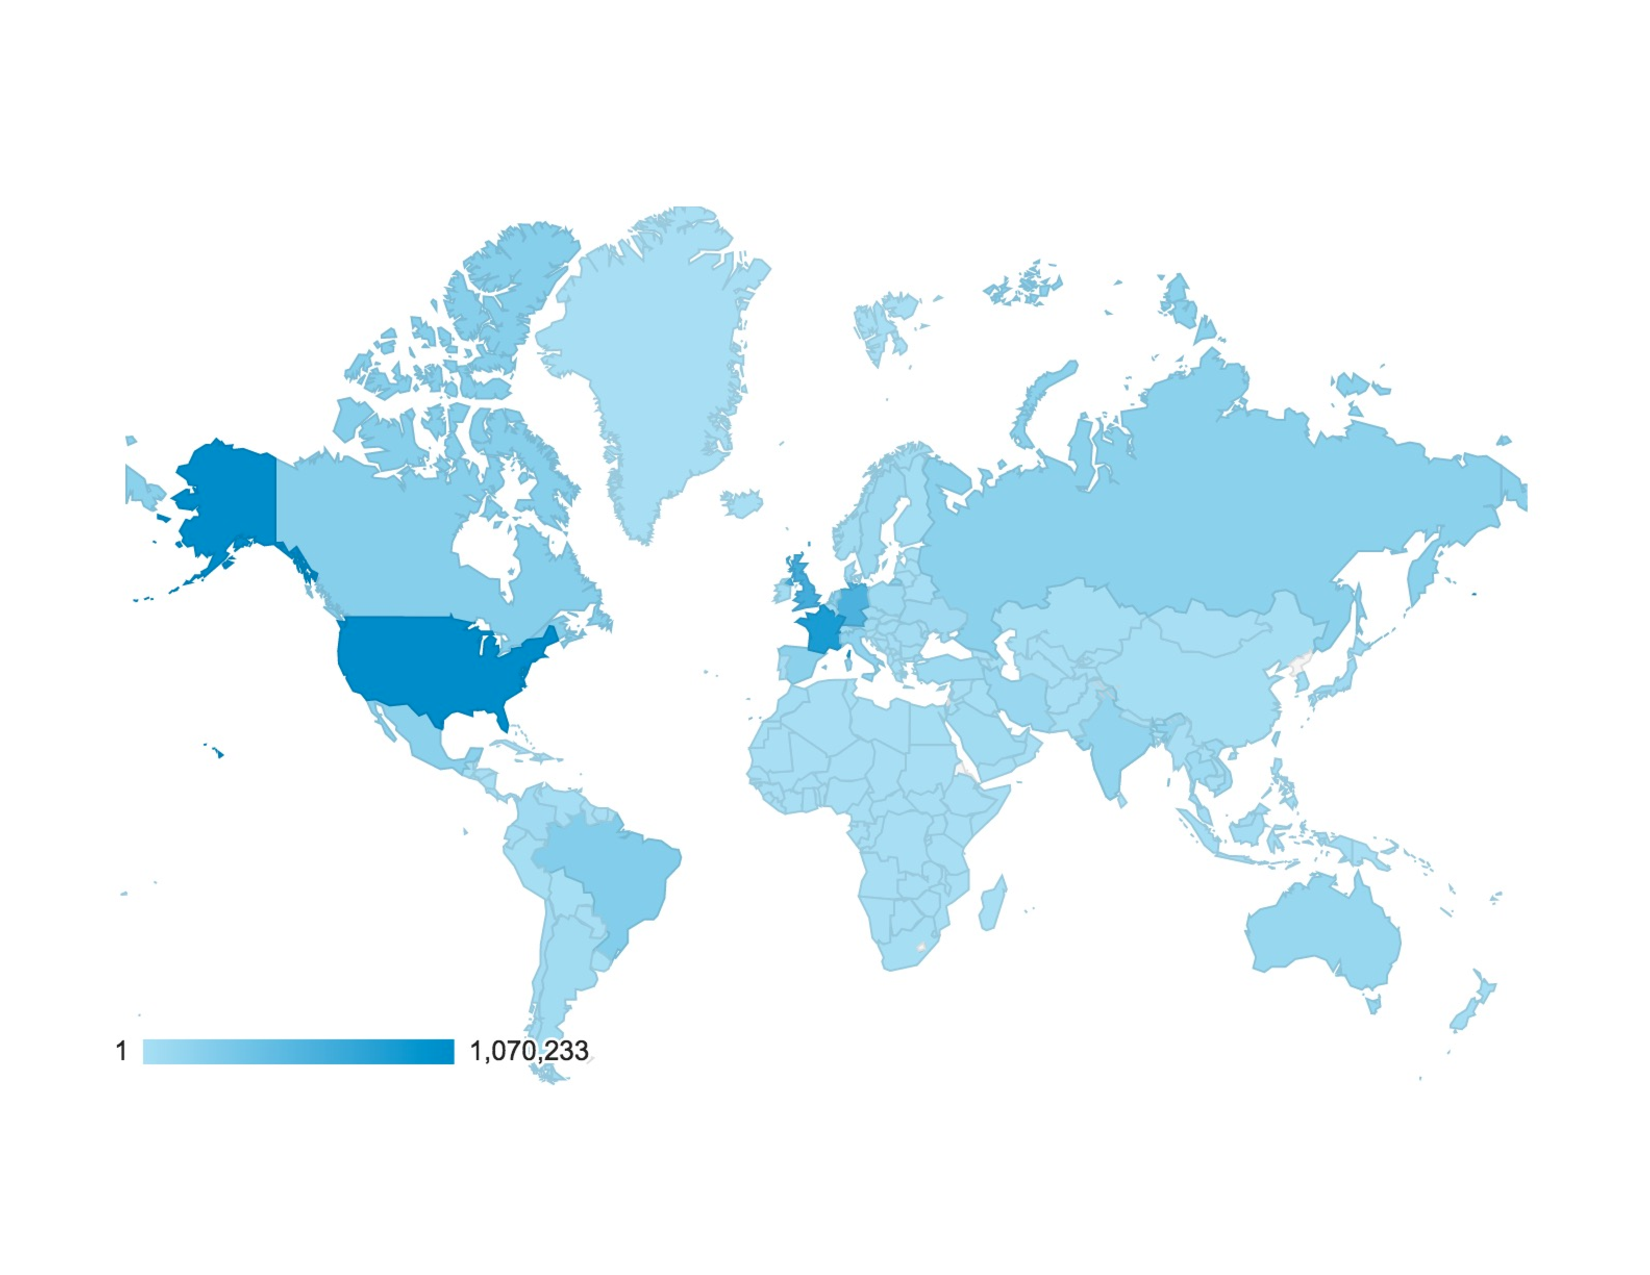
\includegraphics[width=14cm]{charts/session_world_map}
\caption{World map of visits \label{user_map}}
\end{figure}\\
\\
So far, we got ratings from 10253 users, currently the average rating is 3.9 out of 5. The distribution is shown in Figure \ref{ratings}. According to the rating distribution graph, most users are satisfied with our solution and gave 5 stars rating. However, the average rating is heavily influenced by the 1 star rating users. The reason of those unsatisfied users is that it happens that the receiver user have in home is not compatible with our application due to different reasons. It might be protocols are not supported yet, such as Roku box. Network condition problem also contributes to the incompatibility problem, some routers have by default disabled multicast due to security reasons. Another major cause of the incompatibility problem is that even use the same protocol, take DLNA for example, a minor implementation difference may cause the break of connection, thus, in the later phase, we have made receiver specific hacks to make our application work with most DLNA receivers regardless of which implementation they use.\\
\\
\begin{figure}[htb]
\centering 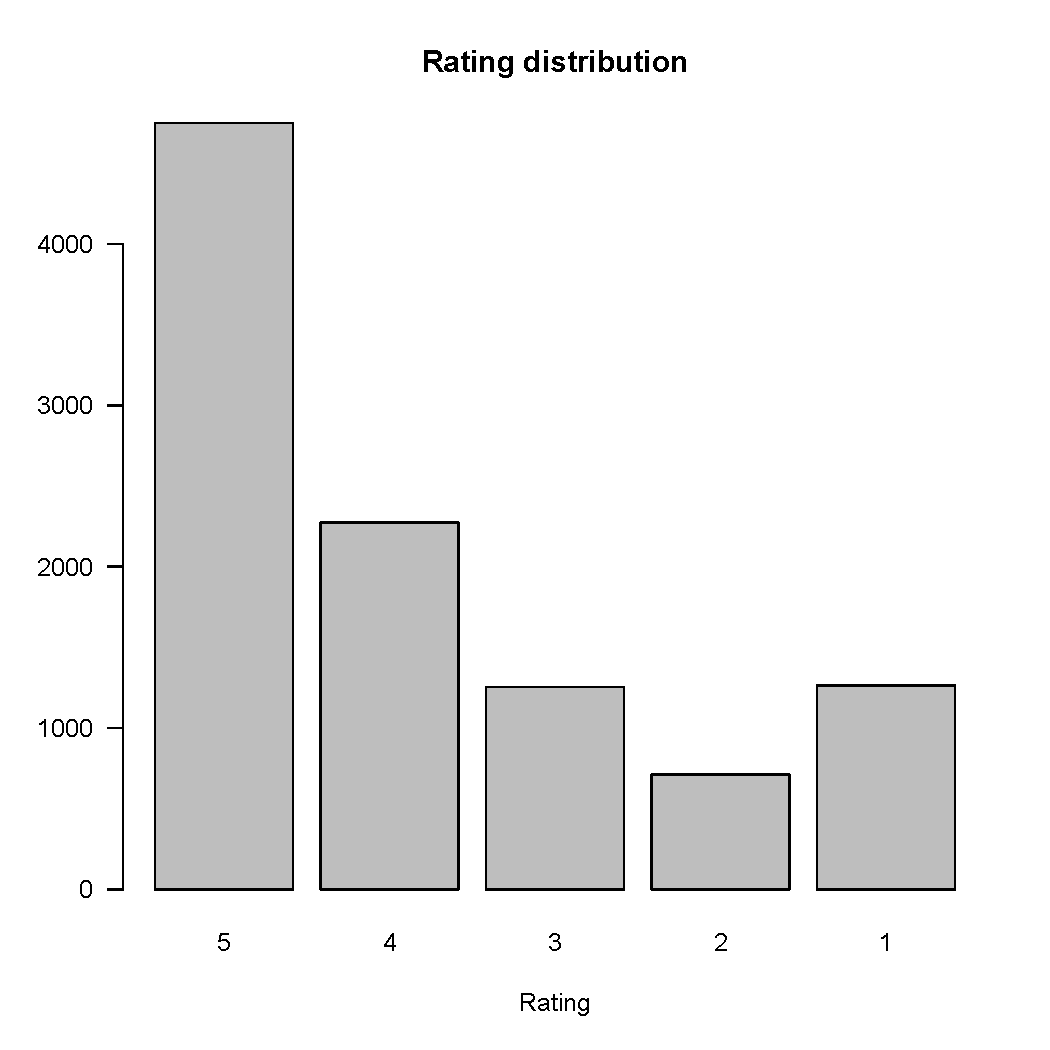
\includegraphics[height=7cm]{charts/rating_distribution}
\caption{Rating distribution\label{ratings}}
\end{figure}\\
\\
In terms of user distribution, in the last 16 months, our application turns out
to be popular in countries like France, United States, Germany, United Kingdom
and Brazil. The user distribution is shown in Figure \ref{user_country}.\\
\\
\begin{figure}[htb]
\centering 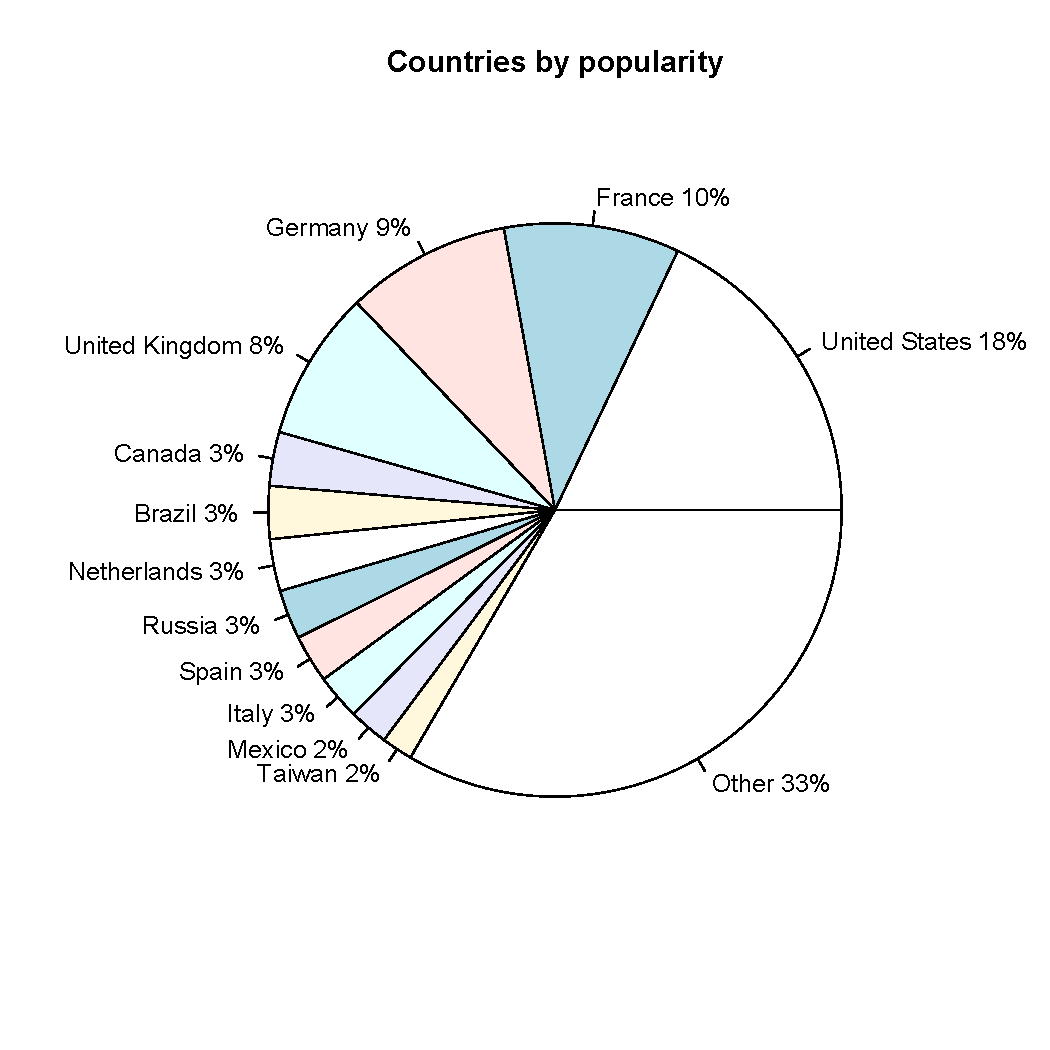
\includegraphics[height=8cm]{charts/country_popularity}
\caption{Popularity in different countries \label{user_country}}
\end{figure}\\
\\
We have also translated the description of our application to nine languages:
 English, Russian, German, Italian, Japanese, French, Chinese, Spanish and Korean. Which may be also an important reason why our users are so international. The application is obviously more popular in European and NorthAmerica countries, that due to the fact that the language of  menu and content is English only and not customized for languages of Asian countries.\\
\\
\begin{figure}[htb]
\centering 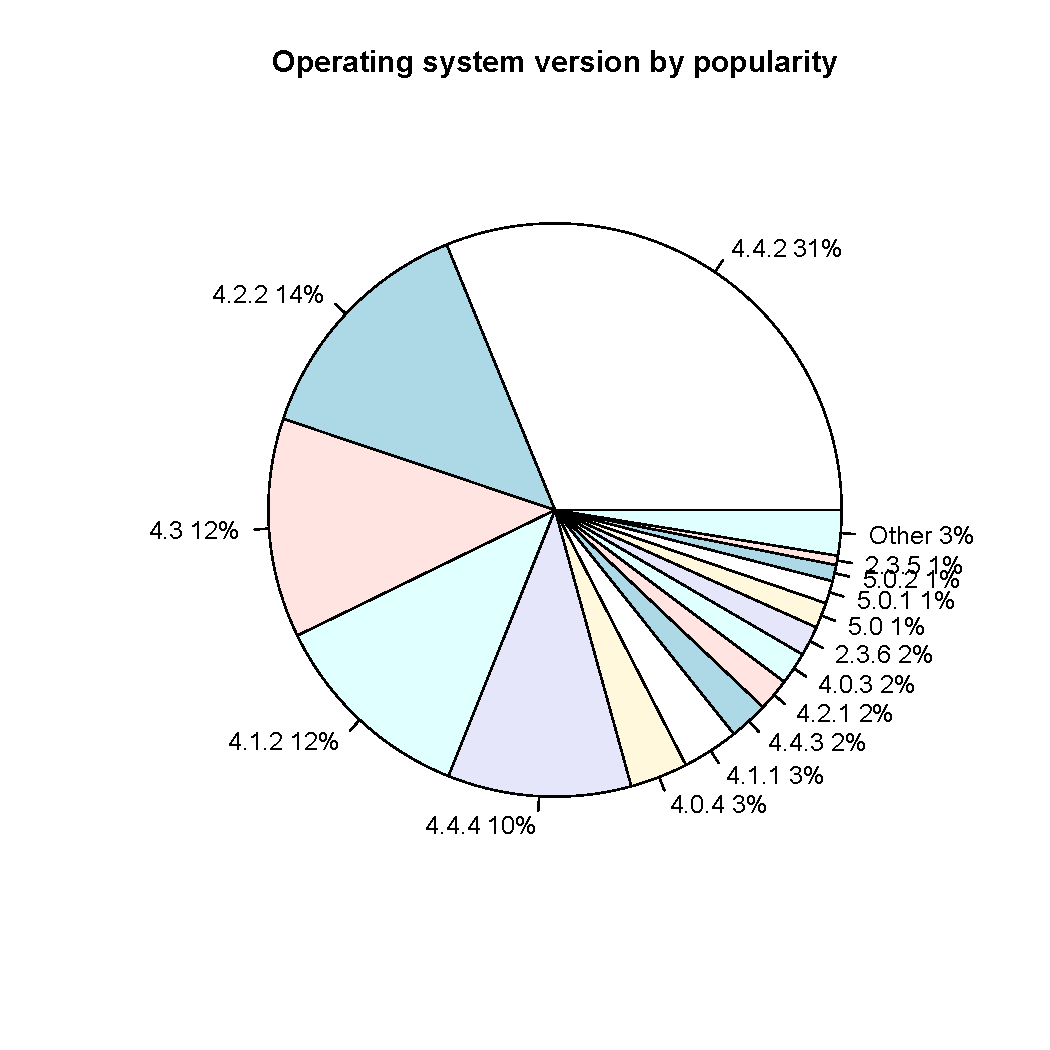
\includegraphics[height=7cm]{charts/os_version_popularity}
\caption{Popularity of different Android versions \label{os_versions}}
\end{figure}\\
\\
The most popular operating system used for our application is Android, but interestingly there are also tens of users was using our application on BlackBerry. Of all the users on Android system, the user distribution is shown in Figure \ref{os_versions}. According to the result, Android Kitkart is the most widely used Android version, which is also our target system version. Most users have updated to latest Kitkart version 4.4. We also have a very small part of users are using latest Android 5.0, who might experience more bugs. The reason is that the latest Android uses Android RunTime (ART) to replace Davik runtime. The native code (C code) support is not optimized so well for the new architecture. But we believe the native code support will be improved in later update of Android Lollipop operating system.\\
\\
The most interesting statistic of our application must be the receiver popularity, which is shown in Figure \ref{receiver_types}. Our project aimed at developing a solution for multimedia home networking, it is especially useful to find out which protocol is the most popular one. According to the result from Google Analytics, the AirPlay and DLNA are the most popular standards, with a combined 87\% of all sessions. Chromecast is the third popular receiver while Amazon Fire TV is the most unpopular receiver. The result also gave us a outlook of the future of multimedia home networking.\\
\\
\begin{figure}[htb]
\centering 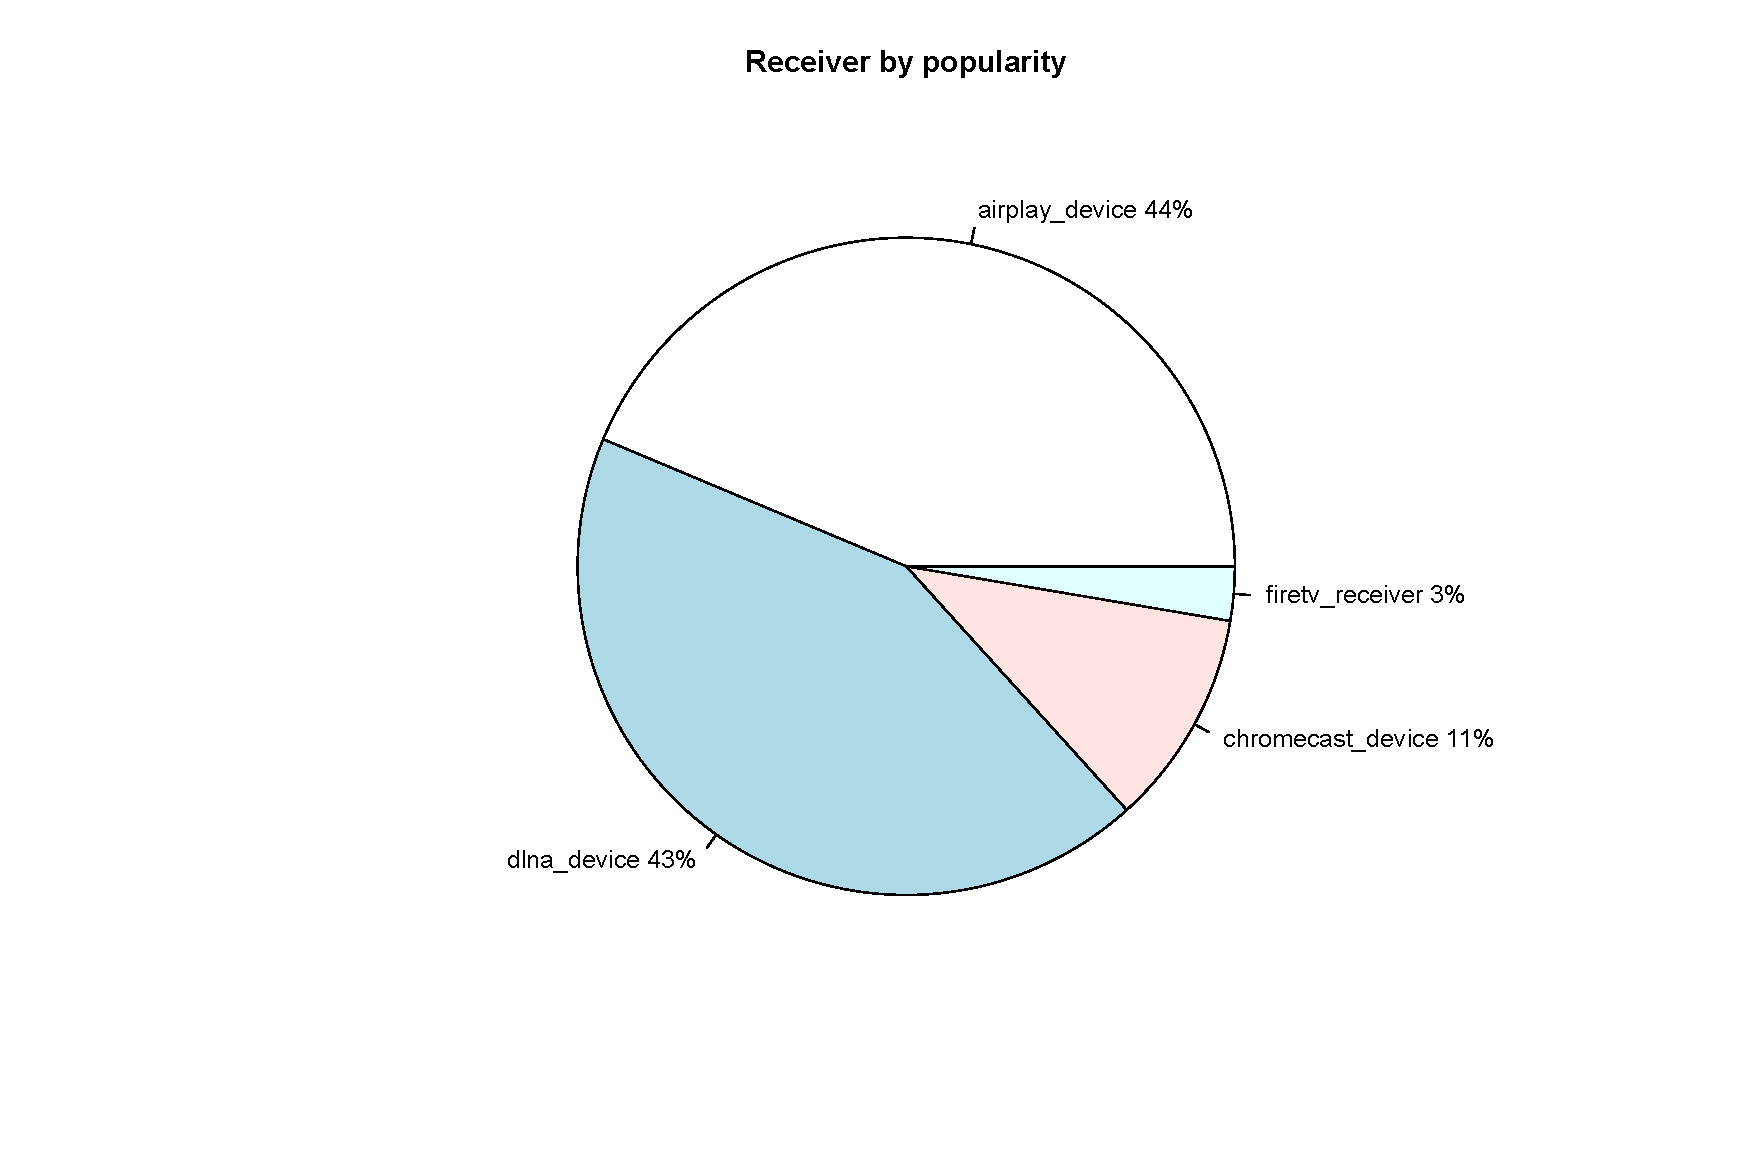
\includegraphics[height=7cm]{charts/receiver_popularity}
\caption{Popularity of receiver types \label{receiver_types}}
\end{figure}
Our application has been public for 16 months, it has received a lot of small updates and one major update in last Christmas. The number of daily visit is shown in Figure \ref{sessions_perday}. As shown in the figure, after the release, the number of users has seen a great increase in the first two months, after that, the number of active users has been steady over the following six months, until we planned a major release after around a year. The new release includes a updated UI and a better written streaming component. Which has brought a significant growth of users, currently our application gets around 40000 daily visits, which has proved our solution has been successful.\\
\\
\begin{figure}[htb]
\centering 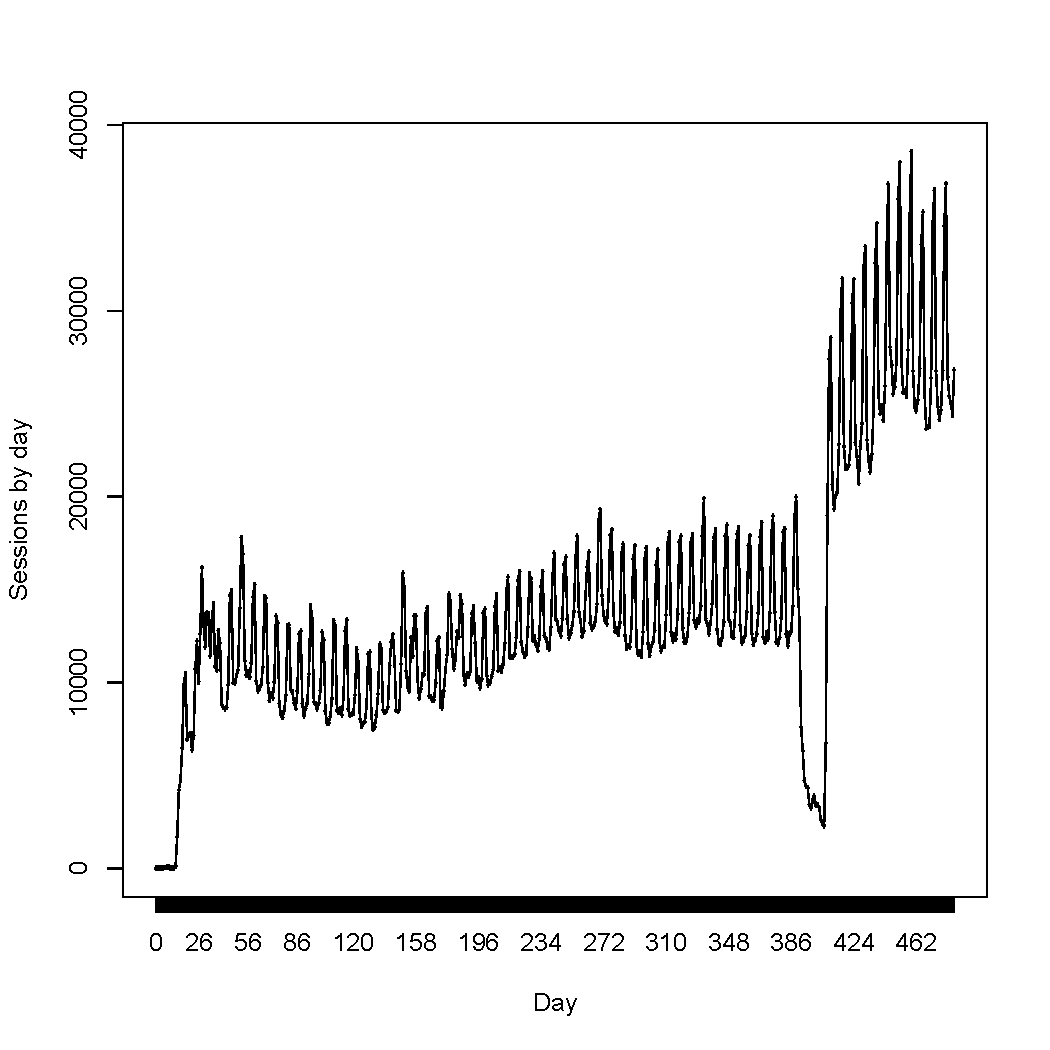
\includegraphics[height=5cm]{charts/sessions_per_day}
\caption{Sessions per day \label{sessions_perday}}
\end{figure}

\subsection{User study}
\begin{itemize}
\item[--]What information we can get back from users
\item[--]User behavior/ statistics
\item[--]Improve the application accordingly
\item[--]Strategies for decision making
\end{itemize}
Write result here.